\documentclass[conference]{sig-alternate-10pt}

%%%%%%%%%%%%%%%%%%%%%%%%%%%%%%%%%%%%%%%%%%%%%%%%%%%%%%%
%%% figure-related settings
\usepackage{graphicx}
\graphicspath{{fig/}, {exp/}}
\DeclareGraphicsExtensions{.pdf,.jpeg,.png,.eps,.jpg}
\usepackage[tight,footnotesize]{subfigure}
%%%%%%%%%%%%%%%%%%%%%%%%%%%%%%%%%%%%%%%%%%%%%%%%%%%%%%%

%%%%%%%%%%%%%%%%%%%%%%%%%%%%%%%%%%%%%%%%%%%%%%%%%%%%%%%
%%% math-algorithm settings
\usepackage{amsmath, amssymb, algorithmic}
\usepackage[lined, boxed, comments numbered, ruled, linesnumbered]{algorithm2e}
%%%%%%%%%%%%%%%%%%%%%%%%%%%%%%%%%%%%%%%%%%%%%%%%%%%%%%%

%%%%%%%%%%%%%%%%%%%%%%%%%%%%%%%%%%%%%%%%%%%%%%%%%%%%%%%
%%% other settings
\usepackage{multirow, longtable, url}
\usepackage{footmisc} % define footref
\usepackage[svgnames, table]{xcolor} % for color
\usepackage{xifthen}% provides \isempty test
\usepackage{setspace}
\usepackage{authblk}% for multiple affiliations of one author 
\usepackage{cite}
\usepackage[font=scriptsize,margin=.5cm]{caption}
\usepackage{color,soul}
\usepackage{xspace}
%\usepackage{calc}
\newcommand{\TODO}[1]{\hl{\textbf{TODO:} #1}\xspace}
\newcommand{\todo}[1]{\TODO{#1}}
\newcommand{\paper}{report~}

\newcommand{\NOTE}[1]{\textcolor{red}{\textbf{NOTE: #1}} \newline}
\newcommand{\FIXME}[1]{\textcolor{red}{\textbf{{FIXME: #1}}} \newline}
\newcommand{\fixme}[1]{\FIXME{#1}}

\newfont{\nicettfont}{cmtt9}
%\newcommand{\ndnName}[1]{``{\nicettfont #1}''}
\newcommand{\schema}[1]{``{\nicettfont #1}''}

\def\UrlBreaks{\do-}
\def\cmd#1{\textit{#1}}
\def\sample#1{\textit{#1}}

%% \name command
%% - allows break before /
\usepackage{etoolbox}
\usepackage{xstring}
\DeclareListParser{\doslashlist}{/}
\newcounter{ndnNameComponentCounter}%
\newcommand{\ndnName}[1]{{%
		\setcounter{ndnNameComponentCounter}{0}%
		\renewcommand{\do}[1]{{%
				\ifnumgreater{\value{ndnNameComponentCounter}}{0}{\allowbreak/}{}%
				\ifnumodd{\value{ndnNameComponentCounter}}{}{}%
				\detokenize{##1}}%
			\stepcounter{ndnNameComponentCounter}}%
		``{\fontfamily{cmtt}\small\selectfont\IfBeginWith{#1}{/}{/}{}\doslashlist{#1}}''%
}}

\def\name#1{\textbf{#1}}
\newcommand{\method}[3][]{%
{\small
\setstretch{0.2}
  \begin{flalign*}
  \ifthenelse{\isempty{#1}}%
    {}% if #1 is empty
    {& \textcolor{DarkGreen}{\mathtt{#1}} &&\\}% if #1 is not empty
     & \begin{aligned}
       \textcolor{DarkBlue}{\fontfamily{pcr}\selectfont
         \textbf{#2}}\textbf{(}#3\textbf{)}
     \end{aligned}&&
  \end{flalign*}
}
}
\newcommand{\argu}[2]{%
  &\textcolor{DarkGreen}{\mathtt{#1}}~#2
}

\newcommand{\nfdconf}[2]{%
{\small
\setstretch{0.2}
  \begin{flalign*}
    &\textcolor{DarkBlue}{\fontfamily{pcr}\selectfont \textbf{#1}}&&\\
    &\begin{aligned} #2 \end{aligned}&&
  \end{flalign*}
}
}

\newcommand{\nfdbra}[2]{%
   &\begin{aligned}
   &\mathtt{#1}\\
   &\{\\
   &~~\begin{aligned}
        #2
      \end{aligned}\\
   &\}
   \end{aligned}\\
}
\newcommand{\nfdv}[2]{%
  &\begin{aligned}
  &\mathtt{#1}~\mathit{#2}\\
  \end{aligned}\\
}
\newcommand{\nfdc}[1]{%
{\small
   $$\mathtt{#1}$$
}
}
%%%%%%%%%%%%%%%%%%%%%%%%%%%%%%%%%%%%%%%%%%%%%%%%%%%%%%%

\usepackage{authblk}

\title{Understanding the Namespace of NDN-Lite}


\begin{document}
\maketitle


\begin{abstract}


\end{abstract}


\section{Introduction}
\label{sec:introduction}

The NDN-Lite library implements the Named Data Networking Stack with the high-level application support functionalities and low-level OS/hardware adaptations for Internet of Things (IoT) scenarios.
NDN-Lite's mainly use cases are the emerging smart homes networks.
We have developed numerous applications based on this framework and will explain how application needs influence the namespace design.

\section{Separate Functionalities}
\label{sec:separation}

We first consider what functionalities a NDN-based home IoT system should provide. 

To serve as a basic NDN entity, one should have four pieces: Name, Certificate, Trust Anchor, and Trust Schema.
We claimed that since they're all first delivered or installed at entities' security bootstrapping time, these trust management should remain in the same sub-namespace.
Then service discovery and access control are needed for the system to faciliate application interaction and content protection, corresponding sub-namespace are needed. 
Considering the independency of the above three functionalities, they should all be kept into non-overlapping subnamespace to avoid conflicts.

Besides basic bricks for a NDN IoT system, common application or devices features should also be considered.
In current smart home systems (cite) devices are often categorized into different capabilities. Applications are represented as consumers for this device provided capabilities.
This style of categorization benefit platform-level Pub/Sub much and become an emerging trend of current IoT systems.
NDN-Lite also follows a similar approach to bring entity's capabilities directly under the root prefix (e.g., \textsl{/alice-home}) to better serve our Pub/Sub~\ref{sec:data-aggregation}.

To summarize, system-level functionalities are separated into different subnamespaces to ease both trust management and data aggregation.
Therefore, NDN-Lite separates overall namespace into following subnamespaces:

\begin{itemize}
\setlength{\itemsep}{0pt}
    \item \textsl{/<home-prefix>/cert}
    \item \textsl{/<home-prefix>/sd}
    \item \textsl{/<home-prefix>/ac>}
    \item \textsl{/<home-prefix>/<capability>}
\end{itemize}

\section{Define Application Data Unit}
\label{sec:application-data-unit}
For NDN applications, it is important to give the definition of Application Data Unit (ADU) as the basic unit of data exchanges.
A clear definition of ADU can help the data transfer be more efficient.
ADU definition should consider \textbf{data producers}, \textbf{data granularity} and \textbf{application semantics}, .

Firstly, for data producer aspect, unclear ADU definition where a single data unit having more than one potential data producers should be avoided. 
Previous work on namespace design ~\cite{liang2018ndnizing} has shown the how data ownership problem of IMAP data structure affect ADU definition in application translation.
However, as a NDN native application, NDN-Lite does not suffer from it and no special design is needed here.
Secondly, data granularity relates to the granularity of data discovery and retransmission thus should be taken carefully to avoid inefficiency.
In the smart home scenario, most data can be abstracted as events, then decision of event-based data granularity comes naturally.
In this case, each ADU represents an event happened within the system, which consists of one or series of Data packets.
Different events (e.g., \textit{turn the fan on} and \textit{close the door}) are categorized into different ADUs and accesssed from diffrent path through the name tree.

Lastly we consider application semantics of ADU. 
The name of ADU should be informational enough to express application semantic, and concise enough to only include application semantics.
Descriptors (e.g., stale or fresh) within the application and not helpful to forwarding should not appear in the ADU's name.
Based this principle, we surveyed mainstream smart home applications ~\cite{smartthings, homekit, awsiot, googlenest} and found essential elements required for constructing a smart home namespace.
\begin{itemize}
    \item \textbf{Capability}: Smart home data are often related with certain platform-level capabilities (e.g., vibration, water leakage detection, pushing SMS notifications).
          The assication should be reflected in names. This idea is aligned with the design decision in Section~\ref{sec:separation}.
    \item \textbf{Data type}: Whether this Data packet refers to a command or content (other prevailing types may exist but out of discussion). 
          The different reliabilty solutions and trust polices can be applied based on data types.
    \item \textbf{Effective scope}: Command type packets issued by applications should contain an scope, and only inside this limited scope commands are effective.
          Similarly, content type packets better adopt this design to avoid confusion. 
          For example, temperature sensed by different sensors in the same room probably vary. 
          Thus names of their produced data should tell the difference of their sensing scope.
    \item \textbf{Command identifier}: Commands can further be categorized based on their semantics, and identifiers are therefore needed.
          Conceptually, commands for \textit{turn the fan off} and \textit{turn the fan on} should be named differently in the case only adult can issue the latter command.
          Such clearness can faciliate access control and trust policy management. 
\end{itemize}
All four elements above should be included into ADU's name, in order to be expressive enough for forwarding and applications performing trust policy examination.
Other less important elements (if any) should be kept out of ADU's name.




\section{Support Aggregation}
\label{sec:data-aggregation}
Namespace should also be designed to support content aggregation, so that applications, at API level, can subscribe to a specific prefix and expect all relevant data below it.
Thus organization the hierarchal name is crucial, given the hierarchy design determines the pattern of aggregation.  

We start determining the hierarchy by making observation that in most cases \textit{effective scope} and \textit{command identifier} are finer granularity of \textit{data type} and \textit{capability}.
Hence the latter two should be at front of the former two.
Then we consider aggregation apporach can benefit application most. 

\begin{figure}[!h]
    \centering
    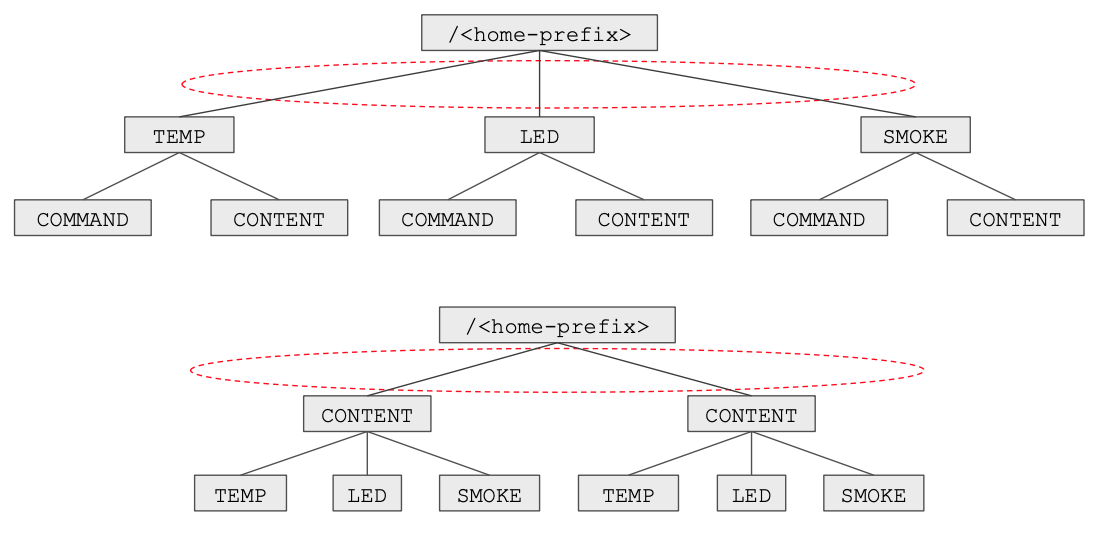
\includegraphics[width=0.5\textwidth]{comparison}
    \caption{Aggregation Approaches Comparison}
    \label{fig:aggregation-comparison}
\end{figure}

Another important observation made is \textit{capability} and \textit{effective scope} are more expressive and providing more data collection dimensions than the other two.
More expressive components should be at smaller depth inside the nametree, to avoid communication overhead of Pub/Sub.
An example is given in Fig~\ref{fig:aggregation-comparison} with three \textit{capability} are invovled. 
One have three dimensiosns of freedom to access namespace from \textsl{/<home-prefix>} when \textit{capability}'s position is upper than \textit{data type}.
In contrast, the other way of aggregation only provide two dimensions of freedom for namespace accessing at the entry point.
In the first organization, received data of subscription on the first depth are either commands or content.
However, data are less guessable when the same subscription happens on the second organization since \textit{capability} has numerous types and more expressive.
Same analysis applies on \textit{effective scope} and \textit{command identifier} situation, and \textit{effective scope} prevails in our application scenarios.

Finally we get the hierarchy which benefits content aggregation most: \textsl{/<home-prefix>/<capability>/<data-type>/<effective-scope>/<data-id>}.
This order also better fit the functionality separation feature in Section~\ref{sec:separation}.
We argue this hierarchy is the outcome of current NDN-Lite applcation needs of accessing namespace with maximized freedom, and this hierarchy may change if applcation needs shift in future.

\section{Putting Together}
\label{sec:putting-together}

The overall namespace of NDN-Lite can be viewed as follows.
In this detailed namespace illustrated in Fig~\ref{fig:overall-namespace}, \textit{Effective scope} are represented with series of name components ranging from zero to two, and timestamp is appened to achieve the Data name uniqueness.

\begin{figure}[!h]
    \centering
    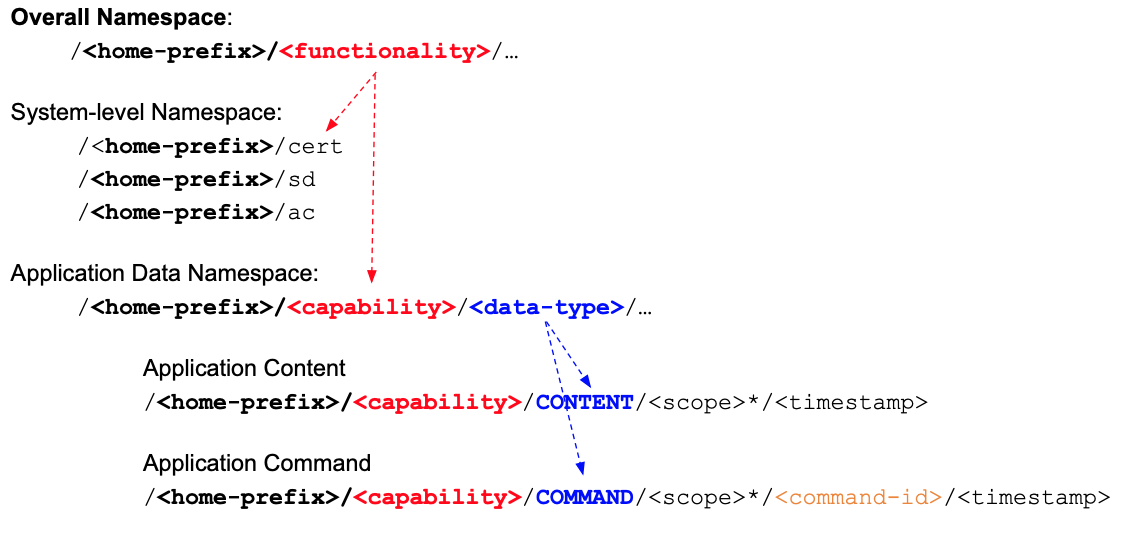
\includegraphics[width=0.5\textwidth]{overall-namespace}
    \caption{Overall NDN-Lite Namespace}
    \label{fig:overall-namespace}
\end{figure}

The last problem not solved is to name identities.
To simplify certificate and trust management, identity names are only allowed binded with one capability.
Multipurpose sensers or applications will host multiple certificates and sign packets with corresponding identities as a result.
Another factor to consider the finest granularity in data publishing.
Content type data, unlike commands often explicitly assigned to an effective scope in data production time, thus need to assign a default fine-grained scope for applications falling back.
We assign this scope in identity names during the bootstrapping time.

\begin{figure}[!h]
    \centering
    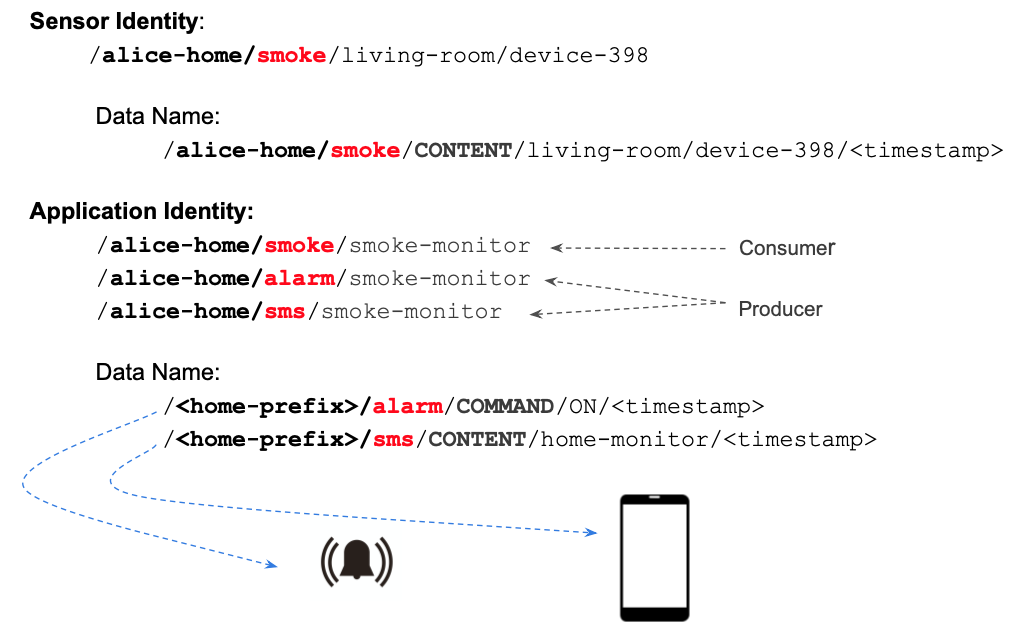
\includegraphics[width=0.5\textwidth]{case-study}
    \caption{Example Application: Smoke Monitor}
    \label{fig:case-study}
\end{figure}

The complete workflow is demonstrated by a case study in Fig~\ref{fig:case-study} with a smoke monitoring application.
Smoke detector installed in the living room is named with \textsl{/alice-home/smoke/living-room/device-398}.
Its encryption key for publishing data under prefix \textsl{/alice-home/smoke} is obtained from access controller residing in \textsl{/alice-home/ac}.
To avoid ambiguities in naming in detection data publishing, data names falls back to \textit{effective-scope} with \textsl{/living-room/device-398}.
The smoke monitor application is installed in the home hub, and three different identities are bootstrapped by this application.
Through subscribing prefix \textsl{/alice-home/smoke}, smoke monitor receive smoke detection data and perform trust schema checking and data decryption.
Its decryption key is obtained from access controller in the same way with smoke detector.
Then two data are published under \textsl{/alice-home/alarm} and \textsl{/alice-home/sms}.
Alarm command issued should be effective in the entire home since not specific \textit{effective-scope} is given.
Meanwhile, user's smartphone which subscribes \textsl{/alice-home/sms} will receive the notification.

\section{Conclusion}
\label{sect:conclusion}

In this \paper, we introduce the namespace of NDN-Lite, the lightweight NDN stack implementation concentrating on smart home scenarios.
Various significant factors are discussed and strong evidence are shown how application needs shape namespace structure.
We will continue udpate this namespace documentation as NDN-Lite's evolution.



\bibliographystyle{abbrv}
\bibliography{reference}

%\appendix
%\input{function}
%\input{instruction}

\end{document}
